% Intended LaTeX compiler: pdflatex
\documentclass[10pt,a4paper,UTF8]{article}
\usepackage{zclorg}
\author{emacsun}
\date{}
\title{Thinking in Java chapter7 笔记和习题}
\hypersetup{
 pdfauthor={emacsun},
 pdftitle={Thinking in Java chapter7 笔记和习题},
 pdfkeywords={},
 pdfsubject={},
 pdfcreator={Emacs 25.0.50.1 (Org mode 9.0.5)}, 
 pdflang={English}}
\begin{document}

\maketitle
\tableofcontents
\titlepic{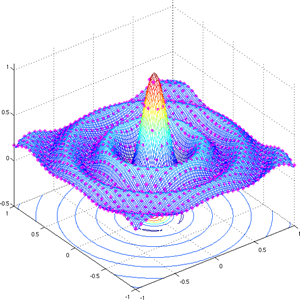
\includegraphics[scale=0.25]{../../img/sinc.PNG}}
像 \texttt{Java} 这样的大型程序语言,每一次升级都牵涉甚广。语言的设计者希望修改语言的某些部分使其效率更高,而语言的使用者希望接口保持不变,从而保证之前的代码能够正常运行。这就产生了矛盾:语言设计者希望修改语言,语言使用者倾向于维持接口不变。于是,语言的设计者必须保证在修改了某些部分之后保持接口不变。对语言使用者来说,语言设计者的修改是透明的。

本章介绍 \texttt{Java} 是如何控制访问权限,从而达到 \texttt{Java} 在升级换代过程中维持函数接口不变的。按照访问权限从高到低排序, \texttt{Java} 提供了 \texttt{package} , \texttt{public} , \texttt{protected} , \texttt{private} 这四个级别的访问控制。其中包访问规定了一组类是如何在一个库中打包的, \texttt{public} \texttt{protected} \texttt{private} 这三个关键词规定了类成员的访问方式。

\section{\texttt{package} :库的最小单元}
\label{sec:org4bbfc20}


一个 \texttt{package} 包含了一组类,这些类在一个命名空间 ( \texttt{namespace} )下。 \texttt{Java} 语言本身内置了很多可用的库,比如 \texttt{utility} 库,这个库在命名空间 \texttt{java.util} 。 \texttt{java.util} 的一个类叫做 \texttt{ArrayList} ,那么我们如何才能使用 \texttt{ArrayList} 呢? 一种可行的方法是使用全名 \texttt{java.util.ArrayList} ,看代码:
\lstset{language=C,label= ,caption= ,captionpos=b,numbers=none}
\begin{lstlisting}
//: access/FullQualification.java
public class FullQualification {
  public static void main(String[] args) {
    java.util.ArrayList list = new java.util.ArrayList();
  }
} ///:~
\end{lstlisting}

然而,使用全名的方法,一看就很烦,名字又臭又长。 \texttt{Java} 提供了一种简单的做法 \texttt{import} 。如果你想要 \texttt{import} 某个特定的类,可以使用 \texttt{import} 语句, 看代码:
\lstset{language=C,label= ,caption= ,captionpos=b,numbers=none}
\begin{lstlisting}
//: access/SingleImport.java
import java.util.ArrayList;
public class SingleImport {
  public static void main(String[] args) {
    ArrayList list = new java.util.ArrayList();
  }
} ///:~
\end{lstlisting}

现在开心了,因为使用 \texttt{ArrayList} 时,不用重复臭长的前缀。但是这样用一个类 \texttt{import} 一个类的方法也不是最有效的,尤其是当我们要用到 \texttt{java.util} 下的好多个类的时候。此时, \texttt{*} 是一个方便的符号,看:
\begin{verbatim}
import java.util.*
\end{verbatim}
这句话把所有的 \texttt{java.util} 下的类都导入了。

\texttt{import} 的做法提供了一种命名空间的管理机制。首先自定义类成员的名字是互相隔离的,比如 类 \texttt{A} 的方法 \texttt{f()} 和类 \texttt{B} 的方法 \texttt{f()} 不会造成冲突(即使他们有相同的签名) 。 那么是不是类成员的名字做到互相隔离就够了呢?不!假设你创建了一个 \texttt{Stack} 类,另外一个人也创建了一个类 \texttt{Stack} ,这个时候怎么办? \texttt{Java} 为这种潜在的冲突提供了完整的解决方案。

截至目前我们都还没有碰到类名冲突的情况,那是因为我们的代码都很简单,当你要和别人一起合作完成较大的项目的时候,做好命名空间的保护是非常必要的。当你编写了一个 \texttt{Java} 文件,这个文件是一个基本的编译单元 ( \texttt{compilation unit} ,有时候也叫 \texttt{translation unit} ) 。每一个编译单元都以 \texttt{.java} 结尾。在这个编译单元中一定有一个 \texttt{public} 类,这个类名必须和文件名字一样(包括大小写!)。 \textbf{在一个编译单元中必须只有一个 \texttt{public} 类,否则的话,编译器会出警告或者报错} 如果在这个编译单元中有多个类,外界是不会知道的,因为他们不是 \texttt{public} 的。这些类为 \texttt{public} 的类提供支持,是幕后的螺丝钉。
\section{组织你的代码}
\label{sec:orgf824f1e}


当你编译 \texttt{.java} 文件时,编译器会为这个文件中的每一个类创建一个文件,这个文件以 \texttt{.class} 结尾。因此编译结束后可能会有相当多的 \texttt{.class} 文件出现在文件夹下面。对于 \texttt{Java} 来说一个可执行的程序就是一堆 \texttt{.class} ,这些 \texttt{.class} 可以通过打包程序生成 \texttt{jar} 文件。在执行的过程中, \texttt{java}  解释器搜寻,装载,解释这些文件。

一个库( \texttt{library} )是一组类文件,每一个源文件包含一个 \texttt{public} 类和任何数量的非 \texttt{public} 类(再次强调,一个文件只有一个 \texttt{public} 类)。如果想要把所有的这些编译单元(也可以说是这些文件)组织在一起,说明他们是一伙的呢? \texttt{package} 关键字就是做这个活的。

在编译单元(不知道我为什么非要称一个源文件为编译单元?好吧,在以后编译单元和一个源文件是等效的。)中使用 \texttt{package} 时,必须把 \texttt{package} 放置到文件的头部,也就是说除了注释意外的第一行。当你说:
\begin{verbatim}
package access;
\end{verbatim}
你在告诉编译器,你在告诉别的程序员:这个编译单元属于一个叫 \texttt{access} 的库。换句话说,这个编译单元的 \texttt{public} 类属于库 \texttt{access} 。这个类的名字被 \texttt{access} 罩着,任何人想要使用这个类都要使用全名或者 \texttt{import} 语句导入这个类,否则无法访问这个类。

举个例子,假设文件名是 \texttt{MyClass.java} 这意味着这个文件中一定有一个 \texttt{public} 类名字是  \texttt{MyClass} 。看代码:
\lstset{language=C,label= ,caption= ,captionpos=b,numbers=none}
\begin{lstlisting}
//: access/mypackage/MyClass.java
package access.mypackage;
public class MyClass {
  // ...
} ///:~
\end{lstlisting}
假若现在有人要用 \texttt{MyClass} 或者 \texttt{access} 中的其他类,他必须用 \texttt{import} 导入或者全名引用,从而使得 \texttt{access} 可以被访问到。


全名引用的做法如下:
\lstset{language=C,label= ,caption= ,captionpos=b,numbers=none}
\begin{lstlisting}
//: access/QualifiedMyClass.java
public class QualifiedMyClass {
  public static void main(String[] args) {
    access.mypackage.MyClass m =
      new access.mypackage.MyClass();
  }
} ///:~
\end{lstlisting}

使用 \texttt{import} 的做法如下:
\lstset{language=C,label= ,caption= ,captionpos=b,numbers=none}
\begin{lstlisting}
//: access/ImportedMyClass.java
import access.mypackage.*;
public class ImportedMyClass {
  public static void main(String[] args) {
    MyClass m = new MyClass();
  }
} ///:~
\end{lstlisting}

\texttt{package} 和 \texttt{import} 可以保证不管多少人在从事同一个 \texttt{Java} 项目都不会造成名字冲突。

\section{创建独一无二的 \texttt{package} 名字}
\label{sec:orgafe17ab}


之前我们看到 \texttt{package} 是如何打包库的: 一个 \texttt{package} 不是把所有的文件合并成一个文件,相反,一个 \texttt{package} 可以由多个 \texttt{.class} 文件构成。那么这些 \texttt{.class} 如何组织?直观简单的做法是:把这些 \texttt{.class} 文件放到一个目录下,即使用操作系统提供的目录结构来组织 \texttt{.class} 文件。 \texttt{Java} 也使用这种方法。

把所有的 \texttt{package} 文件放到一个目录下解决了两个问题:1. 创建了唯一的 \texttt{package} 名字。通过这个目录的路径名字,我们可以找到该 \texttt{package} 的 \texttt{.class} 名字。通常, \texttt{package} 的第一部分是类创建者的域名逆序。由于域名是独一无二的,所以遵循这个规范写的类的名字也是独一无二的。2. 把所有类都保存到一个文件夹下,方便 \texttt{Java} 解释器寻找 \texttt{.class} 文件。


那么,是不是我们用了 \texttt{package} \texttt{import} 以及把类文件放到独一无二的文件路径中就不会有冲突了呢?不是的。假设两个库通过 \texttt{*} 导入,但是这两个库中有同名的类,这该怎么办?
\begin{verbatim}
import net.mindview.simple.*;
import java.util.*;
\end{verbatim}

\texttt{java.util*} 包含了类 \texttt{Vector} ,如果 \texttt{net.mindview.simple.*} 也包含了名为 \texttt{Vector} 的类,怎么办?
\begin{verbatim}
Vector v = new Vector();
\end{verbatim}

上面的一行代码到底调用的是哪里的 \texttt{Vector} 呢?解释器不知道,阅读代码的人也不知道。此时编译器会报错,强制写代码的人修改这个 \texttt{bug} 。如果你想使用 \texttt{java.util.*} 中的 \texttt{Vector} 你必须使用全名导入:
\begin{verbatim}
java.util.Vector v = new java.util.Vector();
\end{verbatim}

了解了 \texttt{package} 和 \texttt{import} 的用法之后,基本上可以编写自己的库了。


\section{\texttt{Java} 访问关键字}
\label{sec:orga9e6f27}


\texttt{java} 提供了 \texttt{public} \texttt{protected} 和 \texttt{private} 三个关键字用于控制对类的访问。这三个关键词控制了类中每一个成员的可访问程度,如果一个类的成员没有提供这三个关键字约束,那么这个成员的访问遵循 \texttt{package access} 也就是说,凡是能访问到这个类所属 \texttt{package} 的都可以访问到这个成员。 不过我们这里不准备再着墨 \texttt{package access} ,因为此前已有不少描述。 \texttt{public} \texttt{protected} 和 \texttt{private} 更值得关注。
\subsection{\texttt{public}}
\label{sec:org4101295}


\texttt{public} 意味着其后面的类成员可以被任何人访问。假设你定义了一个 \texttt{dessert} 类在 \texttt{Cookie.java} 这个编译单元中。看代码:
\lstset{language=C,label= ,caption= ,captionpos=b,numbers=none}
\begin{lstlisting}
//: access/dessert/Cookie.java
// Creates a library.
package access.dessert;
public class Cookie {
  public Cookie() {
    System.out.println("Cookie constructor");
  }
  void bite() { System.out.println("bite"); }
} ///:~
\end{lstlisting}
谨记: \texttt{Cookie.java} 生成的类文件必须在 \texttt{dessert} 的目录下,而 \texttt{dessert} 又必须在 \texttt{access} 所在的目录下,而 \texttt{access} 必须在 \texttt{CLASSPATH} 中包含的路径下。不要错误的默认 \texttt{Java} 会在当前路径下寻找 \texttt{.class} 。如果 \texttt{.} 不在 \texttt{CLASSPATH} 中,那么 \texttt{Java} 不会查看当前目录。现在,我们创建一个使用 \texttt{Cookie} 的程序:
\lstset{language=C,label= ,caption= ,captionpos=b,numbers=none}
\begin{lstlisting}
//: access/Dinner.java
// Uses the library.
import access.dessert.*;
public class Dinner {
  public static void main(String[] args) {
    Cookie x = new Cookie();
    //! x.bite(); // Can’t access
  }
} /* Output:
Cookie constructor
*///:~
\end{lstlisting}

在代码中创建了一个 \texttt{Cookie} 的对象 \texttt{x} ,因为 \texttt{Cookie} 的构造函数是 \texttt{public} 的,这个类是 \texttt{public} 的。但是在 \texttt{Dinner.java} 中不能访问 \texttt{bite()} ,因为 \texttt{bite()} 只能有 \texttt{dessert} 访问(还记得 \texttt{package access} 么?)
\subsection{默认的包}
\label{sec:org6a5f6b8}


下面的代码能够编译通过:
\lstset{language=C,label= ,caption= ,captionpos=b,numbers=none}
\begin{lstlisting}
//: access/Cake.java
// Accesses a class in a separate compilation unit.
class Cake {
  public static void main(String[] args) {
    Pie x = new Pie();
    x.f();
  }
} /* Output:
Pie.f()
*///:~
\end{lstlisting}

第二个文件是:
\lstset{language=C,label= ,caption= ,captionpos=b,numbers=none}
\begin{lstlisting}
//: access/Pie.java
// The other class.
class Pie {
   void f() { System.out.println("Pie.f()"); }
} ///:~
\end{lstlisting}

你可能会以为这两个文件时完全独立的,但是 \texttt{Cake} 却能够创建 \texttt{Pie} 对象,并调用它的成员函数 \texttt{f()} 。他们之所以可以互相访问是因为他们在同一个文件夹中, \texttt{Java} 会把一个文件夹中的文件是做默认的包,因此在一个文件夹下的文件可以互相访问。
\subsection{\texttt{private}}
\label{sec:orgf1fe541}


\texttt{private} 意味着除了这个类之外所有程序都不能访问该成员,包括在同一个 \texttt{package}  的其他类。貌似标记为 \texttt{private} 的类成员隔离了自己,但是细想,如果有很多人在创建同一个 \texttt{package} ,那么这个 \texttt{private} 就有意义了:只有你自己能访问,不用担心会影响到别人。

鉴于 \texttt{pakcage access} 已经提供了一定程度的隔离,你或许会认为 \texttt{private} 不那么重要。错! \texttt{private} 非常重要,尤其在多线程场合(这个会在以后引入,现在只需要知道,该使用 \texttt{private} 的时候一定不要手软)。

\lstset{language=C,label= ,caption= ,captionpos=b,numbers=none}
\begin{lstlisting}
//: access/IceCream.java
// Demonstrates "private" keyword.
class Sundae {
  private Sundae() {}
  static Sundae makeASundae() {
    return new Sundae();
  }
}
public class IceCream {
  public static void main(String[] args) {
    //! Sundae x = new Sundae();
    Sundae x = Sundae.makeASundae();
  }
} ///:~
\end{lstlisting}

上面代码给出了一个使用 \texttt{private} 的例子:有时候你可能想控制一个类的创造过程。在上面的例子中,不能通过 \texttt{Sundae()} 的构造函数来创造类(因为这个构造函数是 \texttt{private} ) ,只能实用 \texttt{makeASundae()} 来创造这个类。

关于 \texttt{private} 的实用有一个准则:任何你觉得是辅助性质的方法都可以标注为 \texttt{private} 。对于类中的数据成员也是如此,除非你要向别人展示类的内部实现,否则类的说有数据域都应该是 \texttt{private} 。
\subsection{\texttt{protected}}
\label{sec:org1f7c1ec}


理解 \texttt{protected} 这个关键词可能需要对 \textbf{继承} 有一点了解。但是为了完整性,这里简单的提一下,继承是根据已有类创建新类的过程。可以再已类的基础上添加新的成员,或者改变已有成员函数的行为。为了继承已有的类,你可以说新类扩展 (extends) 了基类。
\begin{verbatim}
class Foo extends Bar{}
\end{verbatim}

如果新类是基于已有类,那么你可以访问基类的 \texttt{public} 成员。(当然,如果在相同的 \texttt{package} 中,你还可以通过 \texttt{package access} 来访问一些成员 ) 。有时候基类创建者像创建一些只有基类能够访问的成员,而其他类不能访问。 \texttt{protected} 就是做这个活的。 \texttt{protected} 同样提供 \texttt{package access} 也就是说 \texttt{package} 中的其他类也能访问该类中的 \texttt{protected} 成员。
\section{总结}
\label{sec:org566aa60}


本文简要叙述了 \texttt{java} 是如何提供访问控制的。主要包括 使用 \texttt{package} 和 \texttt{import} 来组织库,导入库。使用 \texttt{public} \texttt{protected} 和 \texttt{private} 来控制类成员的访问。
\end{document}
